
\begin{figure*}
  \vspace{-0.1in}
  \centering
  \begin{subfigure}[b]{0.15\textwidth}
    \begin{tikzpicture}[
        spy using outlines={%
          rectangle,magnification=3,size=\textwidth,
          every spy on node/.append style={transparentwindow}
        }
      ]
      \node (figA) at (0.0,0.0) {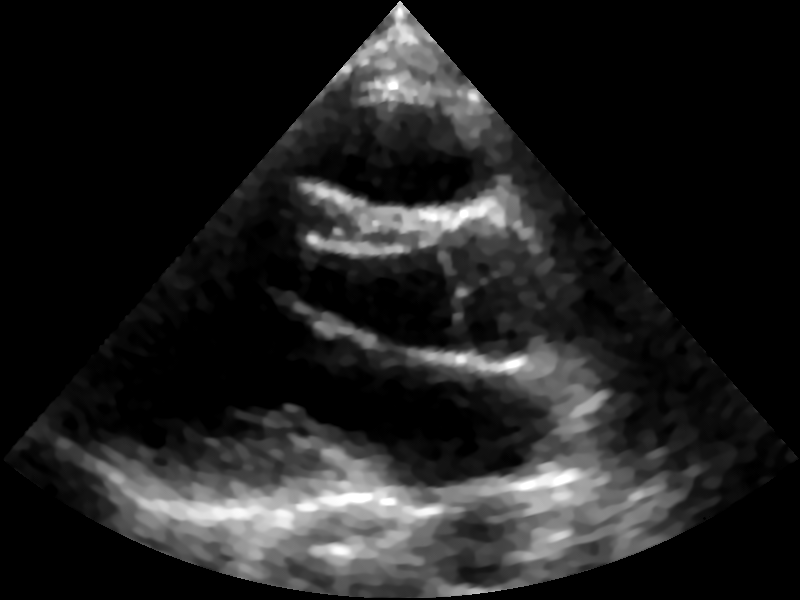
\includegraphics[width=\textwidth]{figures/cardiac1_osrad.png}};
      \spy on (0.05, 0.05) in node [redwindow, anchor=north] at ($(figA.south)$);
    \end{tikzpicture}
    \caption{OSRAD}
  \end{subfigure}%
  \begin{subfigure}[b]{0.15\textwidth}
    \begin{tikzpicture}[
        spy using outlines={%
          rectangle, magnification=3,size=\textwidth,
          every spy on node/.append style={transparentwindow}
        }
      ]
      \node (figA) at (0.0,0.0) {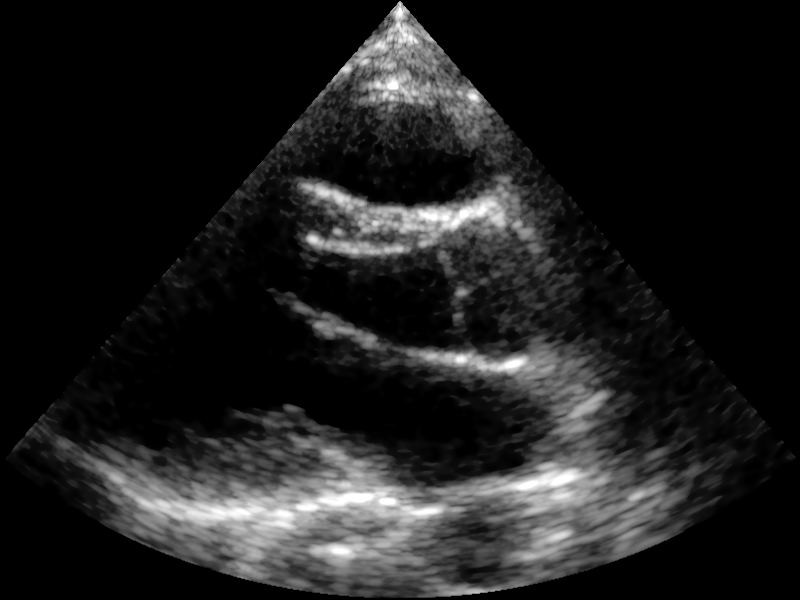
\includegraphics[width=\textwidth]{figures/cardiac1_admss.png}};
      \spy on (0.05, 0.05) in node [redwindow, anchor=north] at ($(figA.south)$);
    \end{tikzpicture}
    \caption{ADMSS}
  \end{subfigure}%
  \begin{subfigure}[b]{0.15\textwidth}
    \begin{tikzpicture}[
        spy using outlines={%
          rectangle, magnification=3,size=\textwidth,
          every spy on node/.append style={transparentwindow}
        }
      ]
      \node (figA) at (0.0,0.0) {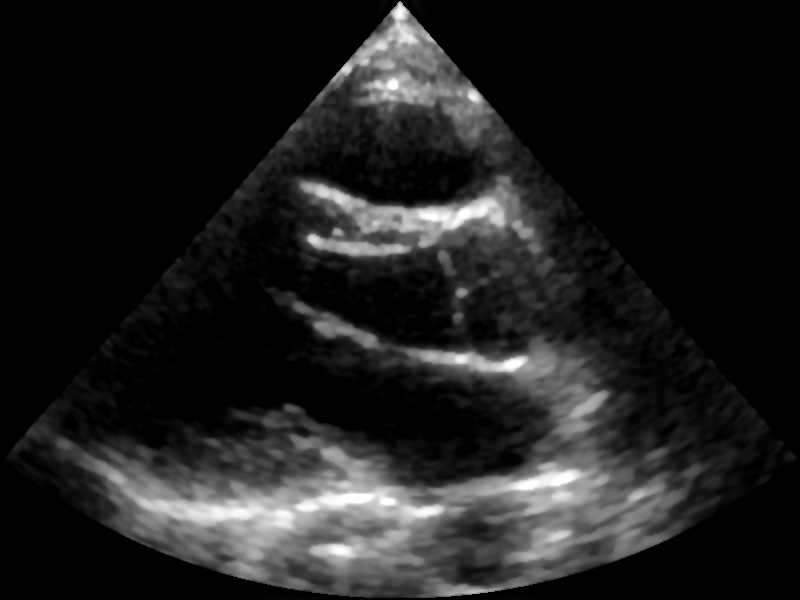
\includegraphics[width=\textwidth]{figures/cardiac1_lpndsf.png}};
      \spy on (0.05, 0.05) in node [redwindow, anchor=north] at ($(figA.south)$);
    \end{tikzpicture}
    \caption{LPNDSF}
  \end{subfigure}%
  \begin{subfigure}[b]{0.15\textwidth}
    \begin{tikzpicture}[
        spy using outlines={%
          rectangle,magnification=3,size=\textwidth,
          every spy on node/.append style={transparentwindow}
        }
      ]
      \node (figA) at (0.0,0.0) {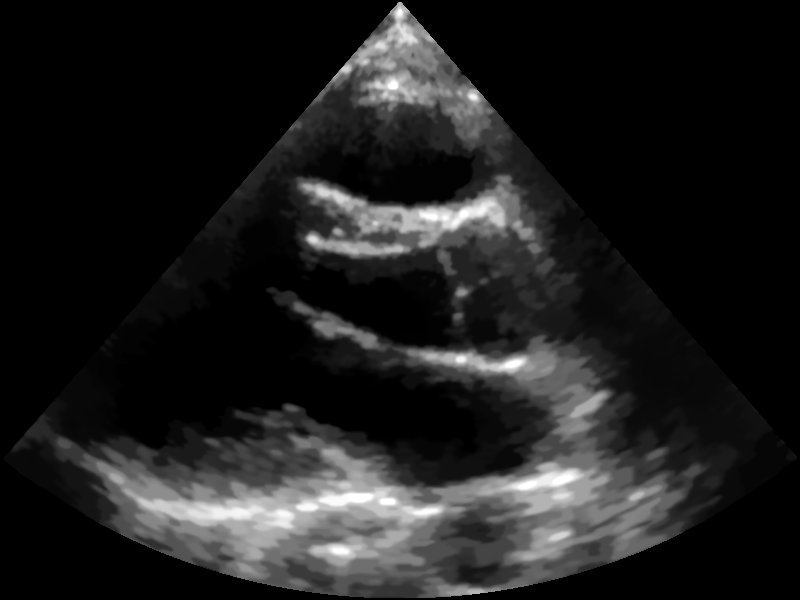
\includegraphics[width=\textwidth]{figures/cardiac1_mnlm.png}};
      \spy on (0.05, 0.05) in node [redwindow, anchor=north] at ($(figA.south)$);
    \end{tikzpicture}
    \caption{MNLM}
  \end{subfigure}%
  \begin{subfigure}[b]{0.15\textwidth}
    \begin{tikzpicture}[
        spy using outlines={%
          rectangle,magnification=3,size=\textwidth,
          every spy on node/.append style={transparentwindow}
        }
      ]
      \node (figA) at (0.0,0.0) {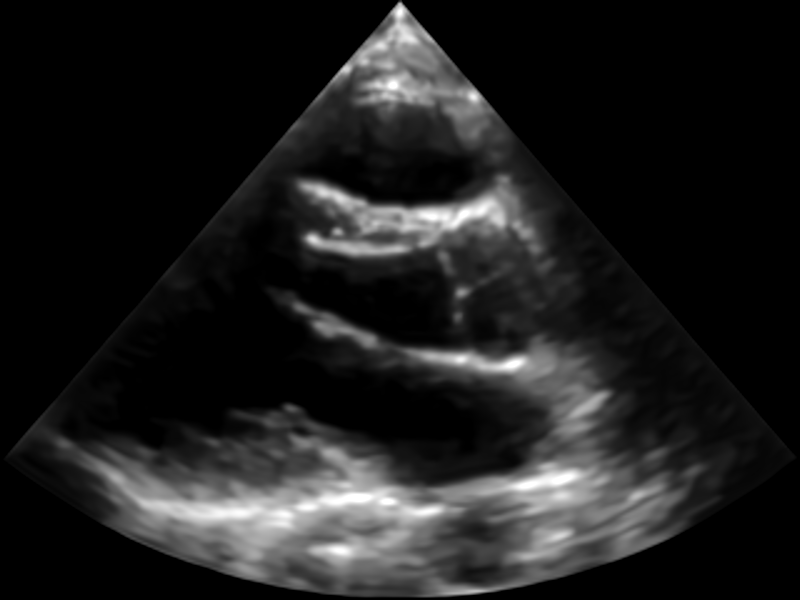
\includegraphics[width=\textwidth]{figures/cardiac1_nllr.png}};
      \spy on (0.05, 0.05) in node [redwindow, anchor=north] at ($(figA.south)$);
    \end{tikzpicture}
    \caption{NLLR}
  \end{subfigure}%
  \begin{subfigure}[b]{0.15\textwidth}
    \begin{tikzpicture}[
        spy using outlines={%
          rectangle,magnification=3,size=\textwidth,
          every spy on node/.append style={transparentwindow}
        }
      ]
      \node (figA) at (0.0,0.0) {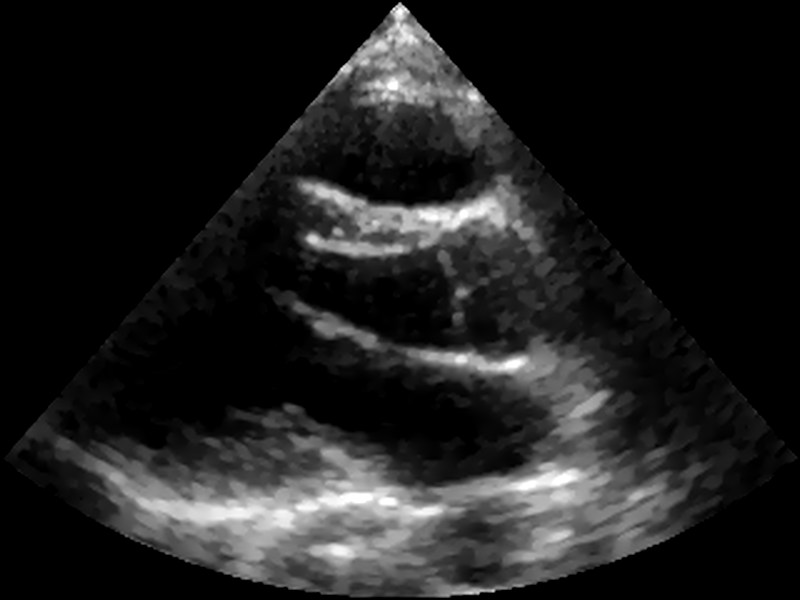
\includegraphics[width=\textwidth]{figures/cardiac1_pfdtv.png}};
      \spy on (0.05, 0.05) in node [redwindow, anchor=north] at ($(figA.south)$);
    \end{tikzpicture}
    \caption{PFDTV}
  \end{subfigure}\\
  %% \begin{subfigure}[b]{0.15\textwidth}
  %%   \begin{tikzpicture}[
  %%       spy using outlines={%
  %%         rectangle,magnification=3,size=\textwidth,
  %%         every spy on node/.append style={transparentwindow}
  %%       }
  %%     ]
  %%     \node (figA) at (0.0,0.0) {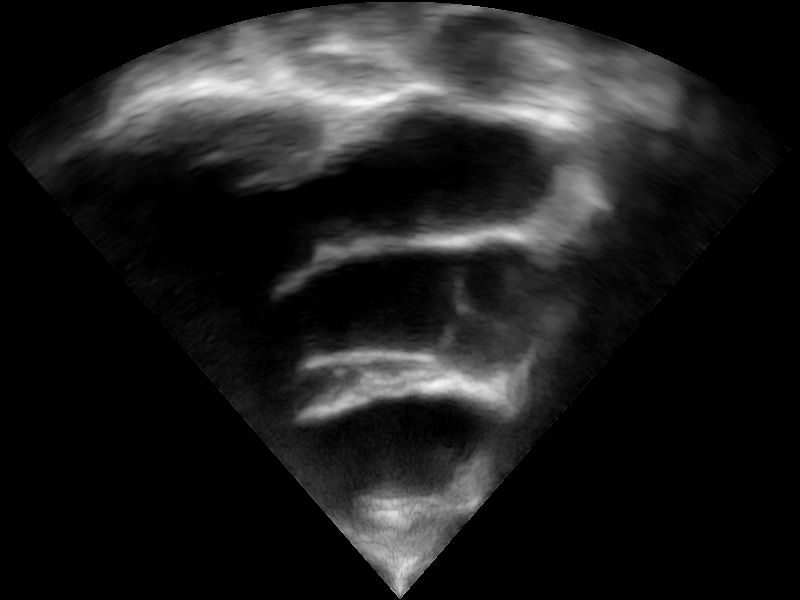
\includegraphics[width=\textwidth, trim={4cm 4cm 4cm 0cm}, clip]{figures/cardiac1_clpdQ.png}};
  %%     \spy on (0.05, 0.05) in node [redwindow, anchor=north] at ($(figA.south)$);
  %%   \end{tikzpicture}
  %%   \caption{CLPD-SSNR}
  %% \end{subfigure}%
  \begin{subfigure}[b]{0.15\textwidth}
    \begin{tikzpicture}[
        spy using outlines={%
          rectangle,magnification=3,size=\textwidth,
          every spy on node/.append style={transparentwindow}
        }
      ]
      \node (figA) at (0.0,0.0) {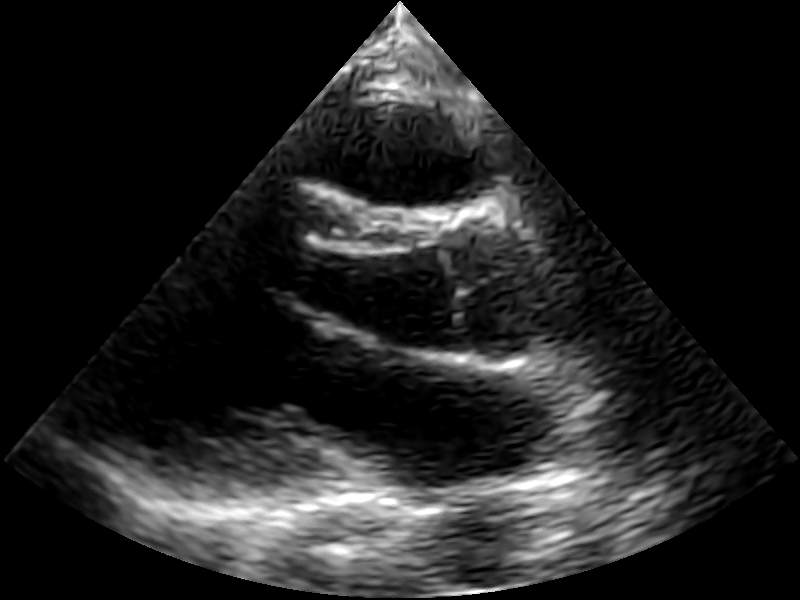
\includegraphics[width=\textwidth]{figures/cardiac1_clpda.png}};
      \spy on (0.05, 0.05) in node [redwindow, anchor=north] at ($(figA.south)$);
    \end{tikzpicture}
    \caption{CLPD-A}
  \end{subfigure}%
  \begin{subfigure}[b]{0.15\textwidth}
    \begin{tikzpicture}[
        spy using outlines={%
          rectangle,magnification=3,size=\textwidth,
          every spy on node/.append style={transparentwindow}
        }
      ]
      \node (figA) at (0.0,0.0) {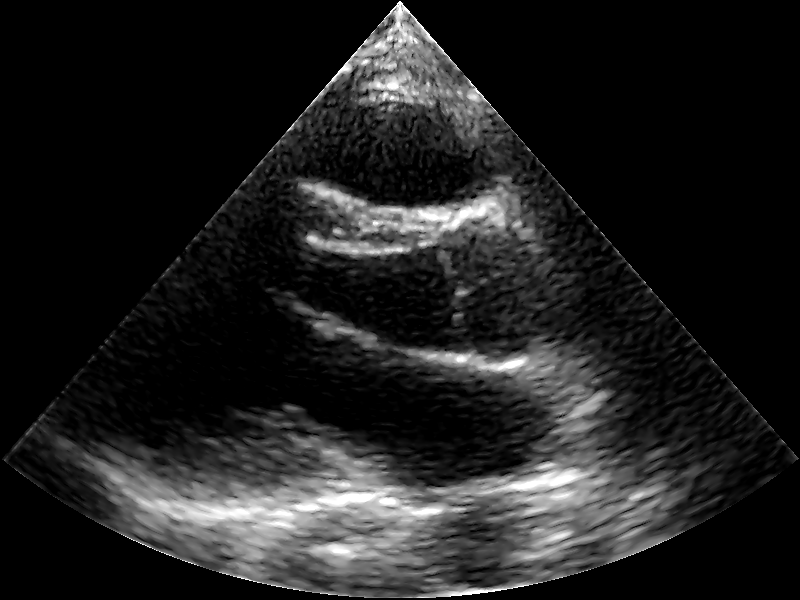
\includegraphics[width=\textwidth]{figures/cardiac1_clpdb.png}};
      \spy on (0.05, 0.05) in node [redwindow, anchor=north] at ($(figA.south)$);
    \end{tikzpicture}
    \caption{CLPD-B}
  \end{subfigure}%
  \begin{subfigure}[b]{0.15\textwidth}
    \begin{tikzpicture}[
        spy using outlines={%
          rectangle,magnification=3,size=\textwidth,
          every spy on node/.append style={transparentwindow}
        }
      ]
      \node (figA) at (0.0,0.0) {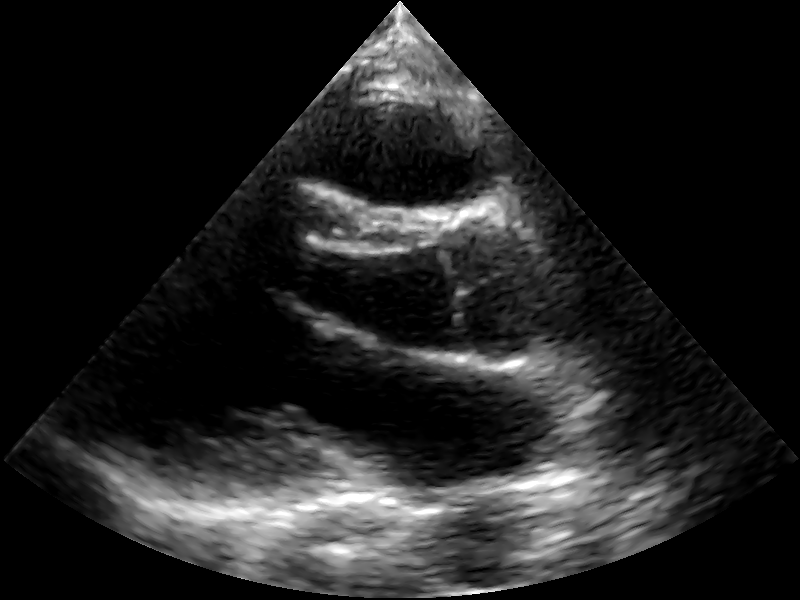
\includegraphics[width=\textwidth]{figures/cardiac1_clpdc.png}};
      \spy on (0.05, 0.05) in node [redwindow, anchor=north] at ($(figA.south)$);
    \end{tikzpicture}
    \caption{CLPD-C}
  \end{subfigure}%
  \begin{subfigure}[b]{0.15\textwidth}
    \begin{tikzpicture}[
        spy using outlines={%
          rectangle,magnification=3,size=\textwidth,
          every spy on node/.append style={transparentwindow}
        }
      ]
      \node (figA) at (0.0,0.0) {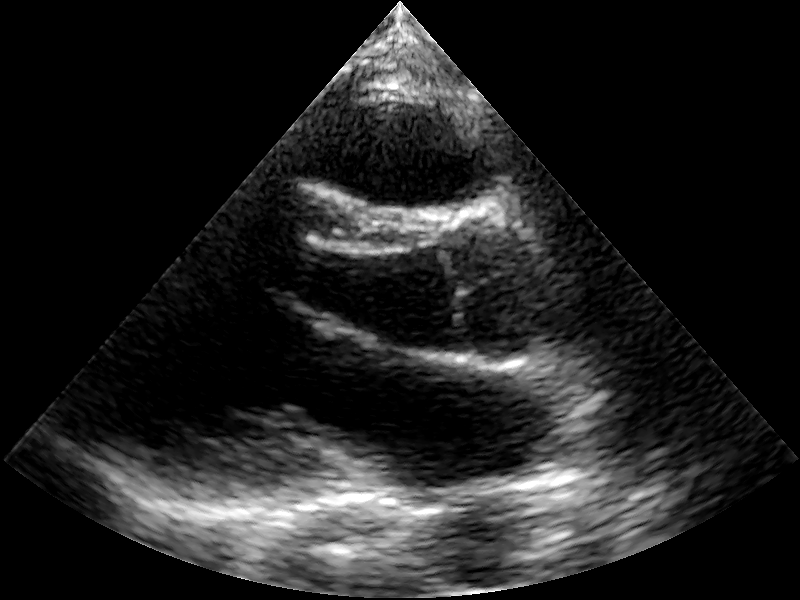
\includegraphics[width=\textwidth]{figures/cardiac1_clpdd.png}};
      \spy on (0.05, 0.05) in node [redwindow, anchor=north] at ($(figA.south)$);
    \end{tikzpicture}
    \caption{CLPD-D}
  \end{subfigure}%
  \begin{subfigure}[b]{0.15\textwidth}
    \begin{tikzpicture}[
        spy using outlines={%
          rectangle,magnification=3,size=\textwidth,
          every spy on node/.append style={redwindow}
        }
      ]
      \node (figA) at (0.0,0.0) {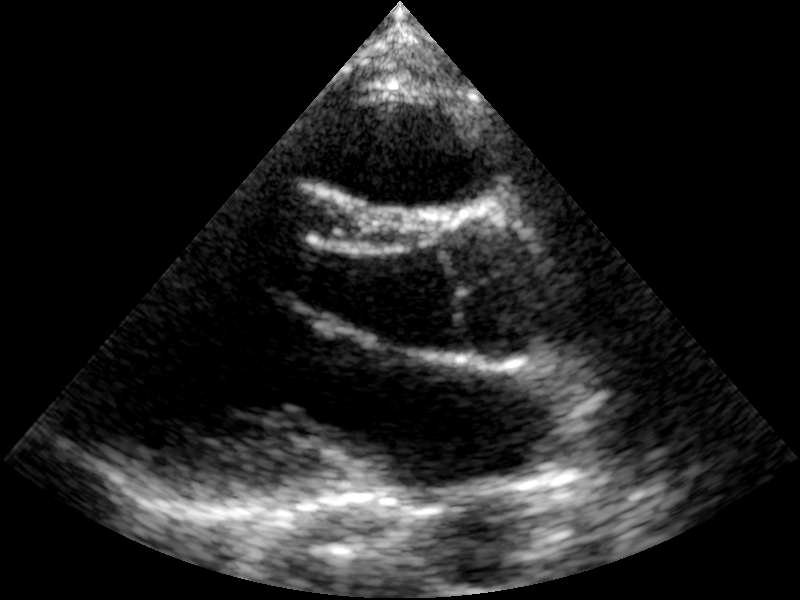
\includegraphics[width=\textwidth]{figures/cardiac1.png}};
      \spy on (0.05, 0.05) in node [redwindow, anchor=north] at ($(figA.south)$);
    \end{tikzpicture}
    \caption{Original}
  \end{subfigure}
  \caption{Results on echocardiography parasternal long-axis view.}\label{fig:cardiac1}
  \vspace{-0.1in}
\end{figure*}

%%% Local Variables:
%%% TeX-master: "master"
%%% End:
